\documentclass[11pt]{article}

\usepackage{amsmath}
\usepackage{amsfonts} 
\usepackage{amsthm}
\usepackage{blkarray}
\usepackage{caption}
\usepackage{enumitem} 
\usepackage{mathtools}
\usepackage{tikz}
\usepackage[top=2cm,bottom=2cm,left=2cm,right=2cm,marginparwidth=1.75cm]{geometry}
\setlength{\parindent}{0cm}

\newcommand{\R}{\mathbb{R}}
\newcommand\simpleGraph[1]{
  \begin{tikzpicture}[every node/.style={circle,draw}]
    \node (a) at (0,1) {};
    \node (b) at (1,1) {};
    \node (c) at (1,0) {};
    \node (d) at (0,0) {};

    \foreach \from/\to in {#1}
      \draw (\from) -- (\to);
  \end{tikzpicture}\hfil
}
\newcommand\itm[1]{\item[\textbf{#1}]}
\newcommand{\incid}{{-}\!{\bullet}\!{-}}
\newcommand{\n}{\vspace{0.5cm}}

\def\lc{\left\lceil}   
\def\rc{\right\rceil}
\def\lf{\left\lfloor}   
\def\rf{\right\rfloor}

\newtheorem{theorem}{Theorem}

\title{\vspace{-1.0cm}MATH 5707 Homework 1}
\author{Fletcher Gornick}
\date{January 18, 2022}

\begin{document}
\maketitle
\begin{itemize}
  \itm{1.2.4} Show that there are eleven nonisomorphic simple graphs on four vertices.

    \simpleGraph{}
    \simpleGraph{a/b}
    \simpleGraph{a/b,a/d}
    \simpleGraph{a/d,b/c}
    \simpleGraph{a/b,a/c,a/d}
    \simpleGraph{a/d,a/b,b/c}

    \simpleGraph{a/b,a/d,b/d}
    \simpleGraph{a/b,b/c,c/d,d/a}
    \simpleGraph{a/b,b/d,c/d,d/a}
    \simpleGraph{a/b,b/c,c/d,d/a,a/c}
    \simpleGraph{a/b,b/c,c/d,d/a,a/c,b/d}



  \itm{1.2.10} The \textit{\(k\)-cube} is the graph whose vertices are the ordered \(k\)-tuples of 0's and 1's, two vertices being joined if and only if they differ in exactly one coordinate.  Show that the \(k\)-cube has \(2^k\) vertices, \(k 2^{k-1}\) edges and is bipartite.

    \begin{proof}
      any \(k\)-length binary string has \(2^k\) possible combinations (2 choices \(k\) times), so there are clearly \(2^k\) vertices.

      For each vertex represented by a binary string, we can change one bit anywhere in the string producing a new vertex in our set differing in exactly one coordinate, and since it's a \(k\)-length binary string, we know that there are \(k\) different strings of hamming distance 1 from our original.  This tells us that every vertex has degree \(k\) (\(k\)-cube is also \(k\)-regular).

      From theorem 1.1, assuming our graph \(G = (V,E)\), \(|V| = \nu = 2^k\) and \(|E| = \varepsilon\), we know that \(\displaystyle\sum_{v \in V} d_G(v) = 2\varepsilon\), so we can plug in \(d_G(v) = k\) for each \(v \in G\), because \(G\) is \(k\)-regular, giving us \(2^k \cdot k = \displaystyle\sum_{v \in V} k = \displaystyle\sum_{v \in V} d_G(v) = 2\varepsilon\).  This tells us that the \(k\)-cube has \(k \cdot 2^{k-1}\) edges.

      Finally, to show the \(k\)-cube is bipartite, we can split the vertices into groups \(V_1\) and \(V_2\).  \(V_1\) will consist of all the vertices with an even \textit{parity} (number of 1's in it's tuple representation), and \(V_2\) will consist of vertices with an odd parity.  Clearly, vertices can only be adjacent to eachother if they have differing parities (otherwise they would be the same vertex, or their hamming distance would be \(\geq 2\)), so the only edges that can exist (in a \(k\)-cube) go between \(V_1\) and \(V_2\).  Thus the \(k\)-cube must be bipartite.
    \end{proof}



  \itm{1.2.11} \begin{enumerate}[label=(\alph*)]
      \item The \textit{complement} \(G^c\) of a simple graph \(G\) is the simple graph with vertex set \(V\), two vertices being adjacent in \(G^c\) if and only if they are not adjacent in \(G\). Describe the graphs \(K^c_n\) and \(K^c_{m,n}\). \n

        The graph of \(K_n^c\) is just the empty graph with \(n\) vertices.  Since every vertex is adjacent to another in \(K_n\), none are in it's complement. \n

        For the graph of \(K_{m,n}^c\), it will consist of two edge-distinct complete graphs \(K_m\) and \(K_n\).  
        \begin{proof}
          First split \(K_{m,n}\) into two subsets \(V_m\) and \(V_n\).  Since \(K_{m,n}\) is a complete bipartite graph, every node in \(V_m\) is adjacent to every node in \(V_n\), therefore none are in it's complement.  Finally, since no vertex in \(V_m\) is adjacent to another in \(V_m\), every vertex is adjacent to every other vertex in it's complement (and similarly for \(V_n\)).  Thus, we get two edge-distinct complete graphs for the complement of a complete bipartite graph.
        \end{proof}

      \item A simple graph \(G\) is \textit{self-complementary} if \(G \cong G^c\). Show that if \(G\) is self-complementary, then \(\nu \equiv 0,1 \pmod 4\)
        \begin{proof}
          A complete graph has \(\displaystyle\binom\nu2\) edges (number of 2-element subsets of \(\{1,2,\hdots,\nu\}\)).  Assuming \(G\) is a spanning subgraph of \(K_\nu\), Then it must be true that \(|E(G)| + |E(G^c)| = |E(K_\nu)| = \displaystyle\binom\nu2 = \frac{\nu(\nu-1)}{2}\).

          For a graph to be self-complementary, it must also be true that \(|E(G)| = |E(G^c)|\) (otherwise \(\varphi \colon E(G) \to E(G^c)\) cannot be bijective), so we can rewrite the above equation to get that \(4|E(G)| = \nu(\nu-1)\)

          Now if \(\nu \equiv 2 \pmod 4\), then \(\nu = 4k+2\) for some \(k \in \mathbb{N}\). So \(\nu(\nu-1) = 4(4k^2 + 3k) + 3\) which is not a multiple of 4.

          For \(\nu \equiv 3 \pmod 4\), \(\nu = 4k+3\) for some \(k \in \mathbb{N}\), meaning \(\nu(\nu-1) = 4(4k^2 + 5k + 1) + 2\).  Again, not a multiple of 4, so unless there's not a whole number of edges, it must be the case that \(\nu \equiv 0,1 \pmod 4\) for a self-complementary graph.
        \end{proof}
    \end{enumerate}



  \itm{1.4.4} Find a bipartite graph that is not isomorphic to a subgraph of any \(k\)-cube.

    \begin{center}
      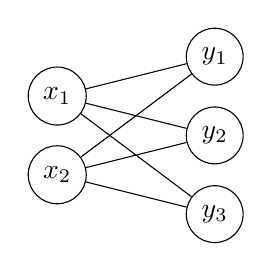
\begin{tikzpicture}[every node/.style={circle,draw}]
        \node (y1) at (0,1.5) {\(x_1\)};
        \node (y2) at (0,0.5) {\(x_2\)};
        \node (x1) at (2,2) {\(y_1\)};
        \node (x2) at (2,1) {\(y_2\)};
        \node (x3) at (2,0) {\(y_3\)};

        \draw (x1) -- (y1) -- (x2) -- (y2) -- (x3) -- (y1);
        \draw (x1) -- (y2);
      \end{tikzpicture}
    \end{center}

    take this bipartite graph for example.  We can denote the vertices of a \(k\)-cube with \(k\)-length binary strings, and edges only connecting vertices with a hamming distance of 1.  We show that 2 distinct vertices cannot be adjacent to the same 3 vertices in any \(k\)-cube.
      \begin{proof}
        Let \(d \colon V^2 \to \mathbb{N} \cup \{0\}\) denote the hamming distance between any two vertices.  if \(d(x_1,x_2) = 0\) then \(x_1 = x_2\), but we wish to deal only with distinct vertices, so assume \(d(x_1,x_2) \geq 1\). \n

        \(d(x_1, x_2) = 1\): In this case we have that \(x_1\) and \(x_2\) are adjacent to eachother.  WLOG, flip any bit in \(x_1\) (excluding the bit flip that leads to \(x_2\)), and call it \(x_3\).  We know \(x_1\) is adjacent to \(x_3\), but \(d(x_2,x_3) = 2\), meaning \(x_1\) and \(x_2\) share no extra adjacent node, so they certainly can't share 3. \n

        \(d(x_1,x_2) = 2\): In this case, \(x_1\) and \(x_2\) differ by two bits.  If we flip either of the bits they differ in (but not both), we get a new vertex adjacent to both \(x_1\) and \(x_2\).  This gives us 2 vertices adjacent to both \(x_1\) and \(x_2\).  But again, WLOG, if we flip any bit other than those two in \(x_1\) and call it \(x_3\), we get that \(d(x_2,x_3) = 3\), so there can exist no more than two nodes adjacent to both \(x_1\) and \(x_2\) in this case. \n

        \(d(x_1,x_2) \geq 3\): Finally, in this case it doesn't matter what bit we flip.  Shifing one bit in \(x_1\) and calling it \(x_3\) results in \(d(x_2,x_3) \geq 2\), so \(x_2\) can never be adjacent to the same node as \(x_1\) with hamming distance \(\geq 3\). \n

        In conclusion, for any \(k\)-cube, two vertices cannot be adjacent to the same 3 vertices, meaning that the above bipartite graph cannot be a subgraph of any \(k\)-cube.
      \end{proof}



  \itm{1.5.5} If \(G\) has vertices \(v_1, v_2, \hdots, v_v\), the sequence \((d(v_1), d(v_2), \hdots, d(v_v))\) is called a \textit{degree sequence} of \(G\).  Show that a sequence (\(d_1, d_2, \hdots, d_n\)) of non-negative integers is a degree sequence of some graph if and only if \(\displaystyle \sum_{i=1}^n d_i\) is even.
    \begin{proof}
      By theorem 1.1, \(\displaystyle\sum_{v \in V} d(v) = 2\varepsilon\), so it's clear that if \((d(v_1), d(v_2), \hdots, d(v_v))\) is a sequence of some graph, it must have an even sum. \n

      Conversely, to show that every degree sequence with even sum can be represented by a graph, we proceed inductively.

      First, suppose we have a degree sequence consisting of just one entry, \(d_1\).  Clearly \(d_1\) must be even, so we can construct a graph consising of \(\displaystyle\frac{d_1}{2}\) loops.

      For any 2-length degree sequence \((d_1,d_2)\), if \(d_1\) and \(d_2\) are both even then we can create a graph where one vertex has \(\displaystyle\frac{d_1}{2}\) loops and the other has \(\displaystyle\frac{d_2}{2}\) loops.  If \(d_1\) and \(d_2\) are odd then we can create a graph where one vertex has \(\displaystyle\frac{d_1-1}{2}\) loops, the other has \(\displaystyle\frac{d_2-1}{2}\) loops, and one link connects the two vertices.

      Now assume every nonnegative degree sequence \((d_1,d_2,\hdots,d_k)\) with \(\displaystyle\sum_{i=1}^{k}d_i\) even is graphic, as well as any smaller degree sequence (strong induction).  We show that every \((k+1)\)-length degree sequence with even sum must also be graphic.

      If \(d_{k+1}\) is even, \(\displaystyle\sum_{i=1}^{k}d_i\) must also be even (otherwise the new sum is odd), so we can just take the graph represented by \((d_1,d_2,\hdots,d_k)\) and add a single node with \(\displaystyle\frac{d_{k+1}}{2}\) loops and we're done.

      Otherwise, if \(d_{k+1}\) is odd, \(\displaystyle\sum_{i=1}^{k}d_i\) must also be odd.  This tells us that at least one of the degrees in \((d_1,d_2,\hdots,d_k)\) is odd as well, call it \(d_j\) (\(1 \leq j \leq k\)).  Now construct a new \((k-1)\)-length sequence consisting of all degrees in our \((k+1)\)-length sequence excluding \(d_j\) and \(d_{k+1}\).  Our new \((k-1)\)-length sequence now has an even sum, so it's graphic by our inductive hypothesis.  We can also create (length 2) sequence \((d_j, d_{k+1})\) with even sum, so it must be graphic as well.  Finally, we can just take the union of the two distinct graphs represented by our two sequences to get a new graph represented by degree sequence \((d_1,d_2,\hdots,d_{k+1})\). \n

      Therefore, by the principle of strong mathematical induction, every \(k\)-length degree sequence with even sum is graphic, so the statement above must hold.
    \end{proof}


  \itm{1.5.7(a)} Let \(\textbf{d} = (d_1, d_2, \hdots, d_n)\) be a nonincreasing sequence of non-negative integers, and denote the sequence \((d_2-1, d_3-1, \hdots, d_{d_1+1}-1, d_{d_1+2}-1, \hdots, d_n)\) by \(\textbf{d'}\).  Show that \(\textbf{d}\) is graphic if and only if \(\textbf{d'}\) is graphic.

  \begin{proof}
    Assume \textbf{d'} is graphic.  We can add vertex \(v_1\) adjacent to the vertices corresponding to \(d_2-1,\hdots,d_{d_1+2}-1\) and rearrange into nonincreasing order to yield degree sequence \textbf{d}. \n

    Conversely, we show that if \textbf{d} is graphic, then \textbf{d'} is as well.  So assume \(\textbf{d} = (d_1, d_2, \hdots, d_n)\) is the degree sequence of some graph \(G\), and \(d_i = d_G(v_i)\) for \(1 \leq i \leq |V(G)|\).

    If \(v_1\) of degree \(d_1\) is adjacent to vertices \(v_2, v_3, \hdots, v_{d_1+2}\), then removing \(v_1\) (and it's incident edges) from \(G\) yields a graph with degree sequence \textbf{d'} and we're done.

    Otherwise, if \(v_1\) isn't adjacent to the next \(d_1\) vertices, we can alter our graph \(G\) to make it this way (without changing the degree sequence).

    Assume \(v_1\) adjacent to vertex \(v_j\) with \(v_j \not\in \{v_2, v_3, \hdots, v_{d_1+2}\}\).  Since \(v_j\) isn't in our initial sequence, there must also exist vertex \(v_i\) in our sequence that's not adjacent to \(v_1\).  We know \(d_G(v_i) \geq d_G(v_j)\) since our degree sequence is nonincreasing, so we can consider two cases.

    \(d_G(v_i) = d_G(v_j)\): In this case we can simple swap the names of the vertices and our degree sequence stays the same but we now have \(v_1\) adjacent to \(v_i\).

    \(d_G(v_i) > d_G(v_j)\): In this case there must exist vertex \(u\) adjacent to \(v_i\), but not \(v_j\).  Now if we swap the set of edges \(\{v_1v_j, v_iu\}\) with \(\{v_1v_i, v_ju\}\), the degrees of each vertex stay the same.  This tells us the degree sequence doesn't change, but \(v_1\) is now adjacent to \(v_i\).

    Since, for graph \(G\) with degree sequence \textbf{d}, we can alter vertices / edges to construct a graph isomorphic to \(G \setminus \{v_1\}\), the converse statement must be true as well.
  \end{proof}
  



  \itm{1.5.10} The \textit{edge graph} of a graph \(G\) is the graph with vertex set \(E(G)\) in which two vertices are joined if and only if they are adjacent edges in \(G\).  Show that, if \(G\) is simple
    \begin{enumerate}[label=(\alph*)]
      \item the edge graph of \(G\)  has \(\varepsilon(G)\) vertices and \(\displaystyle\sum_{v \in V(G)} \binom{d_G(v)}{2}\) edges;
        \begin{proof}
          Obviously the edge graph of \(G\) (call it \(G'\)) will have \(\varepsilon(G)\) vertices, because our new vertex set is just the edge set of \(G\). \n

          As for the number of edges, let's look at each vertex in the original graph separately.  First, note that each vertex \(v \in V(G)\) is incident to \(d_G(v)\) edges (no loops because \(G\) is simple).  All the edges incident to \(v\) must be adjacent to eachother (by definition).

          Let \(S = \{e \in E(G) \mid e \incid v\}\) be the set of edges incident to \(v\).  The induced subgraph \(G'[S]\) is complete (edges adjacent in \(G\) \(\implies\) vertices adjacent in \(G'\)), so there are \(\displaystyle\binom{d_G(v)}{2}\) edges in \(G'[S]\).

        Finally, since \(G\) is simple, there does not exist any double links, so if 2 edges are adjacent to eachother through one vertex, they cannot be adjacent through another.  This tells us that each of the induced subgraphs of \(G'\) are edge-distinct, meaning 
        \[|E(G')| = \sum_{v \in V} G'[\{e \in E(G) \mid e \incid v\}] = \sum_{v \in V(G)} \binom{d_G(v)}{2}.\]
        \end{proof}
        \newpage
        
      \item the edge graph of \(K_5\) is isomorphic to the complement of the graph featured in exercise 1.2.6.
        \begin{figure}[!ht]
          \begin{minipage}{0.45\textwidth}
            \centering
            \resizebox{!}{4cm}{
              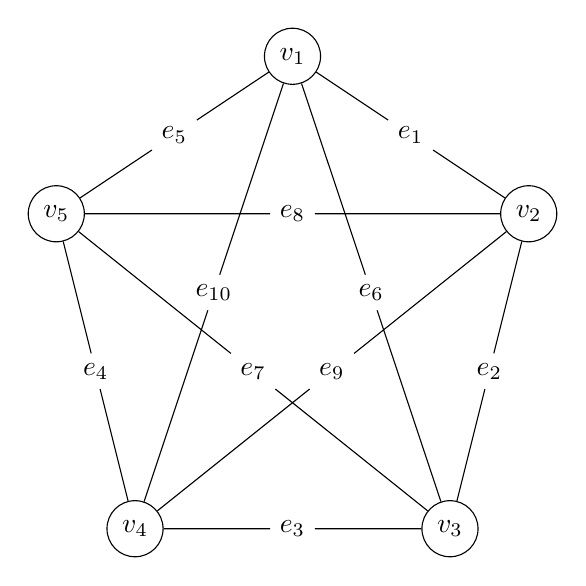
\begin{tikzpicture}
                \node[circle,draw] (v1) at (3,6) {\(v_1\)};
                \node[circle,draw] (v2) at (6,4) {\(v_2\)};
                \node[circle,draw] (v3) at (5,0) {\(v_3\)};
                \node[circle,draw] (v4) at (1,0) {\(v_4\)};
                \node[circle,draw] (v5) at (0,4) {\(v_5\)};

                \node (e1) at (4.5,5) {\(e_1\)};
                \node (e2) at (5.5,2) {\(e_2\)};
                \node (e3) at (3,0) {\(e_3\)};
                \node (e4) at (0.5,2) {\(e_4\)};
                \node (e5) at (1.5,5) {\(e_5\)};

                \node (e6) at (4,3) {\(e_6\)};
                \node (e7) at (2.5,2) {\(e_7\)};
                \node (e8) at (3,4) {\(e_8\)};
                \node (e9) at (3.5,2) {\(e_9\)};
                \node (e10) at (2,3) {\(e_{10}\)};

                \draw (v1) -- (e1) -- (v2) -- (e2) -- (v3) -- (e3) -- (v4) -- (e4) -- (v5) -- (e5) -- (v1);
                \draw (v1) -- (e6) -- (v3) -- (e7) -- (v5) -- (e8) -- (v2) -- (e9) -- (v4) -- (e10) -- (v1);
              \end{tikzpicture}
            }
            \captionsetup{labelformat=empty}
            \caption{\(K_5\) graph}
          \end{minipage}
          \(\Longrightarrow\)
          \begin{minipage}{0.45\textwidth}
            \centering
            \resizebox{!}{4cm}{
              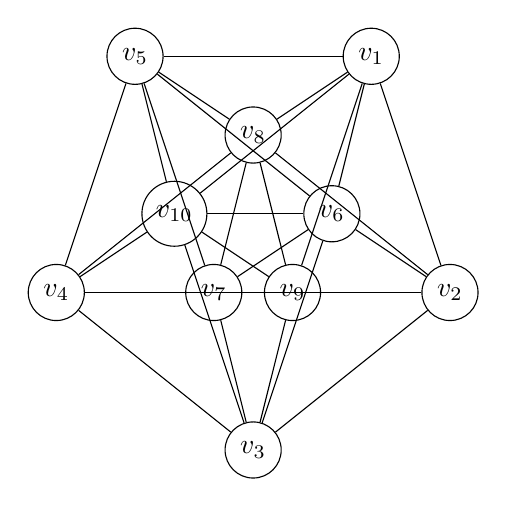
\begin{tikzpicture}
                \node[circle,draw] (v1) at (4.5,5) {\(v_1\)};
                \node[circle,draw] (v2) at (5.5,2) {\(v_2\)};
                \node[circle,draw] (v3) at (3,0) {\(v_3\)};
                \node[circle,draw] (v4) at (0.5,2) {\(v_4\)};
                \node[circle,draw] (v5) at (1.5,5) {\(v_5\)};
                \node[circle,draw] (v6) at (4,3) {\(v_6\)};
                \node[circle,draw] (v7) at (2.5,2) {\(v_7\)};
                \node[circle,draw] (v8) at (3,4) {\(v_8\)};
                \node[circle,draw] (v9) at (3.5,2) {\(v_9\)};
                \node[circle,draw] (v10) at (2,3) {\(v_{10}\)};

                \foreach \from/\to in {v9/v10,v8/v9,v7/v8,v6/v10,v6/v7,v5/v10,v5/v8,v5/v7,v5/v6,v4/v10,v4/v9,v4/v8,v4/v7,v4/v5,v3/v10,v3/v9,v3/v7,v3/v6,v3/v4,v2/v9,v2/v8,v2/v7,v2/v6,v2/v3,v1/v10,v1/v9,v1/v8,v1/v6,v1/v5,v1/v2}
                  \draw (\from) -- (\to);
              \end{tikzpicture}
              \foreach \nd in {v1,v2,v3,v4,v5,v6,v7,v8,v9,v10}
                \tikz[remember picture,overlay]\coordinate(\nd);
            }
            \captionsetup{labelformat=empty}
            \caption{edge graph of \(K_5\)}
          \end{minipage}
          \vspace{1cm}

          \begin{minipage}{0.45\textwidth}
            \centering
            \resizebox{!}{2.5cm}{
              \begin{blockarray}{ccccccccccc}
                & \(v_1\) & \(v_2\) & \(v_3\) & \(v_4\) & \(v_5\) & \(v_6\) & \(v_7\) & \(v_8\) & \(v_9\) & \(v_{10}\) \\
                \begin{block}{c(cccccccccc)}
                  \(v_1\) & * & 1 & 0 & 0 & 1 & 1 & 0 & 1 & 1 & 1 \\
                  \(v_2\) & * & * & 1 & 0 & 0 & 1 & 1 & 1 & 1 & 0 \\
                  \(v_3\) & * & * & * & 1 & 0 & 1 & 1 & 0 & 1 & 1 \\
                  \(v_4\) & * & * & * & * & 1 & 0 & 1 & 1 & 1 & 1 \\
                  \(v_5\) & * & * & * & * & * & 1 & 1 & 1 & 0 & 1 \\
                  \(v_6\) & * & * & * & * & * & * & 1 & 0 & 0 & 1 \\
                  \(v_7\) & * & * & * & * & * & * & * & 1 & 0 & 0 \\
                  \(v_8\) & * & * & * & * & * & * & * & * & 1 & 0 \\
                  \(v_9\) & * & * & * & * & * & * & * & * & * & 1 \\
                  \(v_{10}\) & * & * & * & * & * & * & * & * & * & * \\
                \end{block}
              \end{blockarray}
            }
            \captionsetup{labelformat=empty}
            \caption{edge graph adjacency matrix}
          \end{minipage}
          \(\Longrightarrow\)
          \begin{minipage}{0.45\textwidth}
            \centering
            \resizebox{!}{2.5cm}{
              \begin{blockarray}{ccccccccccc}
                & \(v_1\) & \(v_2\) & \(v_3\) & \(v_4\) & \(v_5\) & \(v_6\) & \(v_7\) & \(v_8\) & \(v_9\) & \(v_{10}\) \\
                \begin{block}{c(cccccccccc)}
                  \(v_1\) & * & 0 & 1 & 1 & 0 & 0 & 1 & 0 & 0 & 0 \\
                  \(v_2\) & * & * & 0 & 1 & 1 & 0 & 0 & 0 & 0 & 1 \\
                  \(v_3\) & * & * & * & 0 & 1 & 0 & 0 & 1 & 0 & 0 \\
                  \(v_4\) & * & * & * & * & 0 & 1 & 0 & 0 & 0 & 0 \\
                  \(v_5\) & * & * & * & * & * & 0 & 0 & 0 & 1 & 0 \\
                  \(v_6\) & * & * & * & * & * & * & 0 & 1 & 1 & 0 \\
                  \(v_7\) & * & * & * & * & * & * & * & 0 & 1 & 1 \\
                  \(v_8\) & * & * & * & * & * & * & * & * & 0 & 1 \\
                  \(v_9\) & * & * & * & * & * & * & * & * & * & 0 \\
                  \(v_{10}\) & * & * & * & * & * & * & * & * & * & * \\
                \end{block}
              \end{blockarray}
            }
            \captionsetup{labelformat=empty}
            \caption{complement adjacency matrix}
          \end{minipage}
          \vspace{1cm}

          \begin{minipage}{\textwidth}
            \centering
            \resizebox{!}{4cm}{
              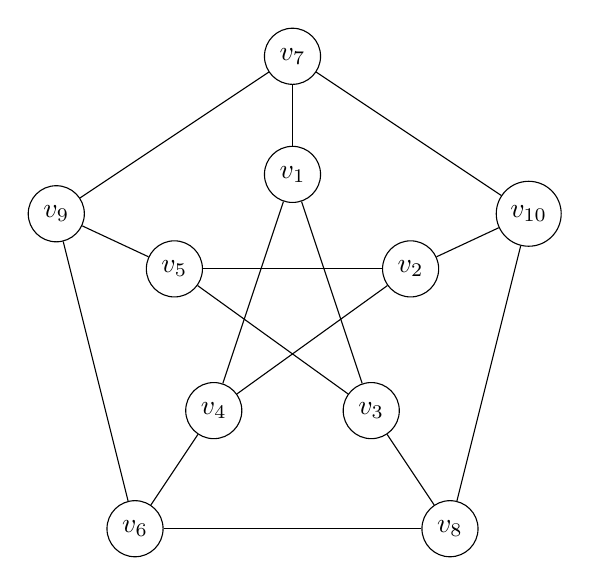
\begin{tikzpicture}
                \node[circle,draw] (v1) at (3,4.5) {\(v_1\)};
                \node[circle,draw] (v2) at (4.5,3.3) {\(v_2\)};
                \node[circle,draw] (v3) at (4,1.5) {\(v_3\)};
                \node[circle,draw] (v4) at (2,1.5) {\(v_4\)};
                \node[circle,draw] (v5) at (1.5,3.3) {\(v_5\)};
                \node[circle,draw] (v6) at (1,0) {\(v_6\)};
                \node[circle,draw] (v7) at (3,6) {\(v_7\)};
                \node[circle,draw] (v8) at (5,0) {\(v_8\)};
                \node[circle,draw] (v9) at (0,4) {\(v_9\)};
                \node[circle,draw] (v10) at (6,4) {\(v_{10}\)};

                \foreach \from/\to in {1/3,1/4,1/7,2/4,2/5,2/10,3/5,3/8,4/6,5/9,6/8,6/9,7/9,7/10,8/10}
                  \draw (v\from) -- (v\to);
              \end{tikzpicture}
            }
            \captionsetup{labelformat=empty}
            \caption{resulting graph (matching the one from 1.2.6)}
          \end{minipage}
        \end{figure}
    \end{enumerate}



  \itm{1.6.7} Show that if \(G\) is disconnected, then \(G^c\) is connected.
    \begin{proof}
      Given any two vertices \(v_1,v_2 \in G\), we show there exists a \((v_1,v_2)\)-path in \(G^c\).

      First, if edge \(v_1v_2 \not\in G\), then \(v_1v_2 \in G^c\), so we've found a path and we're done.

      Now, if \(v_1v_2 \in G\), then they're both in the same component of \(G\), call it \(G'\).  Since \(G\) is disconnected, there are more than one components, so there exists vertex \(v_3 \not\in G'\) with no \((v_1,v_3)\)-path or \((v_2,v_3)\)-path, so there's certainly no \(v_1v_3\) edge or \(v_2v_3\) edge.  This tells us that these edges are certainly in \(G^c\) meaning we can construct a path between \(v_1\) and \(v_2\) by going through \(v_3\).

      Therefore, if \(G\) is disconnected, it's complement is connected.
    \end{proof}
  


  \itm{1.6.10} Show that any two longest paths in a connected graph have a vertex in common.
    \begin{proof}
      Take any graph \(G=(V,E)\) with longest paths \(P,Q\) of lengths \(m,n\) respectively.  Let \(V(P) = \{u_1,u_2,\hdots,u_m\}\) and \(V(Q) = \{v_1,v_2,\hdots,v_n\}\), and suppose, to the contrary, \(V(P) \cap V(Q) = \emptyset\).

      Since \(G\) is connected, for any vertices \(u_i \in P, v_j \in Q\), there must exist some path \(R\) with length \(\geq 1\) connecting \(u_i\) to \(v_j\).  Now consider the subpaths \(P_1 = u_1u_2 \hdots u_i\), \(P_2 = u_{m}u_{m-1} \hdots u_i\), \(Q_1 = v_1v_2 \hdots v_j\), \(P_2 = v_{n}v_{n-1} \hdots v_j\), and take the paths of maximum length \(P_{\text{max}} = \displaystyle\max_{\text{length}} (P_1, P_2)\) and \(Q_{\text{max}} = \displaystyle\max_{\text{length}} (Q_1, Q_2)\).

      From this, we can construct a new path \(P_{\text{max}}RQ_{\text{max}}\), with \[\omega(P_{\text{max}}RQ_{\text{max}}) \geq \lc\frac{\omega(P_{\text{max}})}{2}\rc + 1 + \lc\frac{\omega(Q_{\text{max}})}{2}\rc > \min\left( \omega(Q), \omega(P) \right),\]

      But this contradicts the fact that \(P\) and \(Q\) are maximum-length paths, thus they must have a vertex in common.
    \end{proof}



  \itm{1.7.2} Show that if \(\delta \geq 2\), then \(G\) contains a cycle.
  \begin{proof}
    Suppose, to the contrary, that \(G\) does not contain a cycle.  So there must exist some path of maximum length inside \(G\) starting at \(v_0\).  We know that \(d_G(v_0) \geq 2\), so \(v_0\) is adjacent to \(v_1\) and some other node \(u\).  If this is the case then we can construct a new longer path starting at \(u\), which is a contradiction, so \(G\) must contain a cycle.

    (Note that if \(G\) is a multigraph and contains loops / double links, then we already have a cycle, so this case is trivial.)
  \end{proof}



  \itm{4.1.1} Which of the following figures can be drawn without lifting one's pen from the paper or covering a line more than once?
    \begin{figure}[!ht]
      \begin{minipage}{0.3\textwidth}
        \centering
        \resizebox{!}{4cm}{
          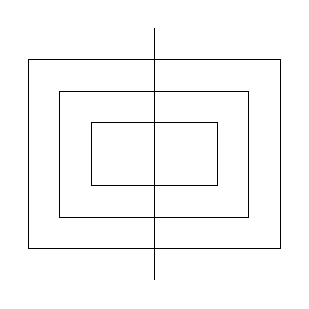
\begin{tikzpicture}[scale=0.4]
            \draw (4,0) -- (4,8);
            \draw (0,1) rectangle (8,7);
            \draw (1,2) rectangle (7,6);
            \draw (2,3) rectangle (6,5);
          \end{tikzpicture}
        }
        \captionsetup{labelformat=empty}
        \caption{(a)}
      \end{minipage}
      \begin{minipage}{0.3\textwidth}
        \centering
        \resizebox{!}{4cm}{
          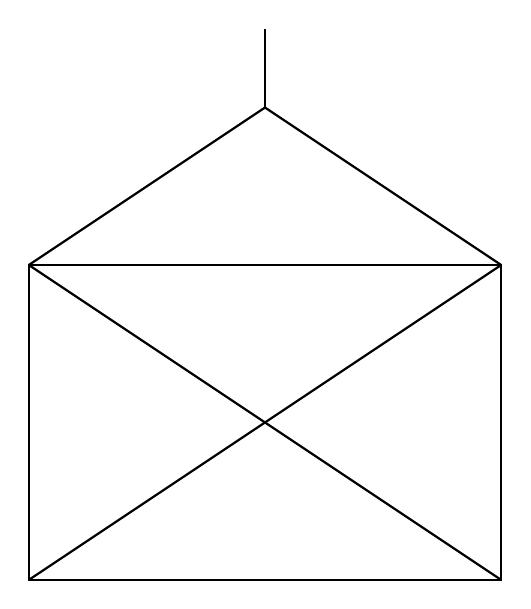
\begin{tikzpicture}
            \draw[thick] (0,0) rectangle (6,4);
            \draw[thick] (0,0) -- (6,4);
            \draw[thick] (0,4) -- (6,0);
            \draw[thick] (0,4) -- (3,6);
            \draw[thick] (6,4) -- (3,6);
            \draw[thick] (3,6) -- (3,7);
          \end{tikzpicture}
        }
        \captionsetup{labelformat=empty}
        \caption{(b)}
      \end{minipage}
      \begin{minipage}{0.3\textwidth}
        \centering
        \resizebox{!}{4cm}{
          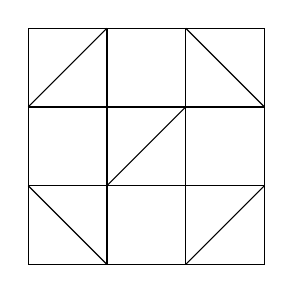
\begin{tikzpicture}
            \draw (0,0) rectangle (3,3);
            \draw (0,1) -- (3,1);
            \draw (0,2) -- (3,2);
            \draw (1,0) -- (1,3);
            \draw (2,0) -- (2,3);
            \draw (0,2) -- (1,3);
            \draw (2,3) -- (3,2);
            \draw (0,1) -- (1,0);
            \draw (2,0) -- (3,1);
            \draw (1,1) -- (2,2);
          \end{tikzpicture}
        }
        \captionsetup{labelformat=empty}
        \caption{(c)}
      \end{minipage}
    \end{figure}

    If we treat each end and intersection point as a vertex, we get the following (nonincreasing) degree sequences:
    \begin{align*}
      (a) &: (4,4,4,4,4,4,2,2,2,2,2,2,2,2,2,2,2,2,1,1) \\
      (b) &: (4,4,3,3,3,1) \\
      (c) &: (5,5,4,4,4,4,4,4,4,4,4,4,2,2,2,2)
    \end{align*}

    The graphs of (a) and (c) both have exactly two vertices of odd degree, so there exists an Euler trail on them.  For (b), there are 4 odd-degree vertices, so no Euler trail exists.  Therefore figures (a) and (c) can be written without lifting one's pen ore repeating a line, but (b) cannot. \n

  \itm{4.1.2} If possible, draw an eulerian graph \(G\) with \(\nu\) even and \(\varepsilon\) odd; otherwise, explain why there is no such graph.
    \begin{center}
      \resizebox{!}{2cm} {
        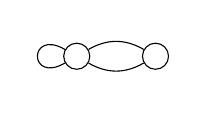
\begin{tikzpicture}[every node/.style={circle,draw}, every loop/.style={in=150,out=210}]
          \node (a) at (0,0) {};
          \node (b) at (1,0) {};

          \draw (a) edge [loop left] (b);
          \draw (a) edge [bend right] (b);
          \draw (a) edge [bend left] (b);
        \end{tikzpicture}\hfil
      }
    \end{center}
    This graph has 2 vertices and 3 edges with a clear Euler tour. \n
  



  \itm{4.2.2} A mouse eats his way through a \(3 \times 3 \times 3\) cube of cheese by tunnelling through all of the 27 \(1 \times 1 \times 1\) subcubes.  If he starts at one corner and always moves on to an uneaten subcube, can he finish at the centre of the cube?

  Assuming there's no diagonal tunneling involved, we can construct a graph with vertices representing each mini-block of cheese adjacent to their immediate (non-diagonal) neighbors.

  Each of the 8 corner blocks are adjacent to exactly 3 edge blocks.  Also each of the 6 center-face blocks connect 4 edge pieces plus the core.  This gives us a total of 14 vertices with odd degree.

  The entire degree sequence of this cheese cube would look like this:
  \[(\overbrace{6}^{\text{core}},\underbrace{5,5,5,5,5,5}_{\text{face-centers}},\overbrace{4,4,4,4,4,4,4,4,4,4,4,4}^{\text{edges}},\underbrace{3,3,3,3,3,3,3,3}_{\text{corners}})\]

  Since there are more than two odd-degree vertices, there exists no path for the mouse by corollary 4.1. \n


  \itm{4.2.3} Show that if \(G\) has a Hamilton path then, for every proper subset \(S\) of \(V\), \(\omega(G-S) \leq |S|+1\).
  \begin{proof}
    If \(G\) has a Hamilton path \(P = v_1e_2v_2e_3 \hdots e_{\nu}v_{\nu}\), then either \(G\) is hamiltonian or we can add an edge connecting the origin and terminus \(v_1v_{\nu}\) making \(G + v_1v_{\nu}\) hamiltonian.

    In the first case, if \(G\) is hamiltonian already, then we know \(\omega(G-S) \leq |S|\) by theorem 4.2, so it's clear that the above statement is true. \n

    Otherwise, if \(S\) is a proper subset of \(V\), then there are again two cases to consider.

    If \(v_1 \in S\), \(v_{\nu} \in S\), or both, the subgraph \((G + v_1v_{\nu}) - S\) doesn't contain \(v_1v_{\nu}\) anyway, so \((G + v_1v_{\nu}) - S = G - S\), thus \(\omega(G-S) \leq |S|\) by 4.2 again.

    Finally, if both \(v_1,v_{\nu} \not\in S\), then \(\omega((G+v_1v_{\nu})-S) \leq |S|\) by 4.2.  Removing the \(v_1v_{\nu}\) edge from our subgraph could potentially split it's component into two smaller components, but if that's the case then \(\omega\) only goes up by 1, so we have that \(\omega(G-S) \leq |S|+1\).
  \end{proof}
  

\end{itemize}

\end{document}
